\section{Ablation Studies}
We present a set of ablations to empirically validate different components of our pipeline:
the technical modifications described in Sec.~\ref{sec:approach}, the pretraining data and the impact of model distillation. 
We consider various downstream tasks that are described in Sec.~\ref{sec:results}.

\subsection{Improved Training Recipe}
\label{sec:ablation-ibot}
Our approach improves over the iBOT method by combining it with several existing components described in Sec.~\ref{sec:approach}.
To evaluate their importance, we train multiple models where we successively add components to a baseline iBOT model.
We report the Top-1 accuracy on the validation set of ImageNet-1k with a k-NN and a linear probe in Table~\ref{tab:ibot-dino}. 
Generally, we observe that each component improves the performance on either k-NN or linear probing and even both in most cases.
Only LayerScale and Stochastic Depth incur a performance drop in linear probing but significantly improve the training stability in our experience.

\begin{table}[t]
  \centering
  \begin{tabular}{@{} l ll @{}}
    \toprule
    & \multicolumn{1}{c}{INet-1k k-NN} & INet-1k linear \\
    \midrule
    iBOT                                    & 72.9                  & 82.3  \\
    ~+(our reproduction)                    & 74.5  \qinc{1.6}    & 83.2  \qinc{0.9}   \\ 
    ~+LayerScale, Stochastic Depth          & 75.4  \qinc{0.9}    & 82.0  \qdec{1.2}   \\ 
    ~+128k prototypes                       & 76.6  \qinc{1.2}    & 81.9  \qdec{0.1}   \\
    ~+KoLeo                                 & 78.9  \qinc{2.3}    & 82.5  \qinc{0.6}   \\ 
    ~+SwiGLU FFN                            & 78.7  \qdec{0.2}    & 83.1  \qinc{0.6}   \\ 
    ~+Patch size 14                         & 78.9  \qinc{0.2}    & 83.5  \qinc{0.4}   \\ 
    ~+Teacher momentum 0.994                & 79.4  \qinc{0.5}    & 83.6  \qinc{0.1}   \\ 
    ~+Tweak warmup schedules                & 80.5  \qinc{1.1}    & 83.8  \qinc{0.2}   \\ 
    ~+Batch size 3k                         & 81.7  \qinc{1.2}    & 84.7  \qinc{0.9}   \\ 
    ~+Sinkhorn-Knopp                        & 81.7  \qeq{}        & 84.7  \qeq{}       \\ 
    ~+Untying heads = \OURS                 & 82.0  \qinc{0.3}    & 84.5  \qdec{0.2}   \\ 
    \bottomrule
  \end{tabular}
  \caption{
    \textbf{Ablation study of the training differences between iBOT and \OURS.} 
We optimize for k-NN performance, as in our experience, the linear probe performance is lower-bounded by the k-NN performance. 
Some modifications, like LayerScale and a high Stochastic Depth (rate=$0.4$), incur a decrease in linear probe performance, but have the benefits of increasing the stability of training by avoiding NaN loss values during training \rone{\citep{touvron2022deit}}.
Overall, these modifications allowed for the next set of improvements to be added. Experiments are run using the ViT-Large architecture on ImageNet-22k.
  }
  \label{tab:ibot-dino}
\end{table}


\subsection{Pretraining Data Source}
The quality of features is directly related to the quality of the pretraining data.
In this experiment, we probe the impact of \LaViDa{} compared to ImageNet-22k, a commonly used pretraining dataset, or using directly raw and uncurated data.
For the uncurated dataset, we randomly sample $142$ million images from the same data source as \LaViDa.
We train a ViT-g/14 on each dataset for the same number of iterations.
We also include a variant of ImageNet-22k obtained by removing the synsets of ImageNet-1k (INet-22k $\setminus$ INet-1k) for completeness.
We report the comparisons in Table~\ref{tab:ablation-data}.

\begin{table}[t]
  \centering
  \begin{tabular}{@{} l c ccccccc @{}}
    \toprule
    Training Data && INet-1k & Im-A & ADE-20k & Oxford-M & \rthree{iNat2018} & \rthree{iNat2021} & \rthree{Places205} \\
    \midrule
    INet-22k                        && \bf 85.9 & 73.5 & 46.6 & 62.5 & \rthree{81.1} & \rthree{85.6} & \rthree{67.0} \\
    INet-22k $\setminus$ INet-1k    && 85.3 & 70.3 & 46.2 & 58.7 & \rthree{80.1} & \rthree{85.1} & \rthree{66.5} \\
    Uncurated data                  && 83.3 & 59.4 & 48.5 & 54.3 & \rthree{68.0} & \rthree{76.4} & \rthree{67.2} \\
    \LaViDa                         && 85.8 & \bf 73.9 & \bf 47.7 & \bf 64.6 & \rthree{\bf 82.3} & \rthree{\bf 86.4} & \rthree{\bf 67.6} \\
    \bottomrule
  \end{tabular}
  \caption{
    \textbf{Ablation of the source of pretraining data.}
    We compare the INet-22k dataset that was used in iBOT to our dataset, \LaViDa.
    Each model is trained for the same number of iterations, that is smaller than in our final run, without high-resolution adaptation.
    Pretraining on \LaViDa{} maintains the performance over INet-1k while leading to models that perform better in other domains.
  }
  \label{tab:ablation-data}
\end{table}



The most salient observation is that training on a curated set of images works better on most benchmarks than training on uncurated data.
This confirms the benefit of curating data, even in the case of self-supervised pretraining.
When compared with models trained on ImageNet-22k, training on \LaViDa{} is also superior on all the benchmarks but ImageNet-1k.
This confirms that training on a more diverse set of images improves the quality of the features in domains that are not covered by \rthree{ImageNet-22k}.
\rthree{We also see that training on our curated data increases the performances on domains that are not used for the curation process (INaturalist 2018, 2021 and Places205), proving that scale and diversity can benefit unseen domains.}
Overall, the conclusion of this ablation is that our dataset provides a good balance of different types of images that leads to the best performance overall.


\subsection{Model Size and Data}
We quantify the importance of scaling data with the model size in Fig.~\ref{fig:scaleperf}.
As the size of models grow, training on \LaViDa\ becomes more beneficial than training on ImageNet-22k.
For instance, a ViT-g trained on \LaViDa\ matches the performance on ImageNet-1k of a model trained on ImageNet-22k while significantly outperforming it on the other benchmarks.  

\begin{figure*}[t]
  \centering
  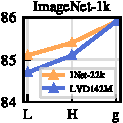
\includegraphics{stamp_ImageNet-1k.pdf}
  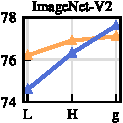
\includegraphics{stamp_ImageNet-V2.pdf}
  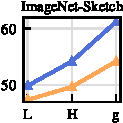
\includegraphics{stamp_ImageNet-Sketch.pdf}
  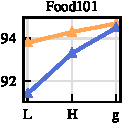
\includegraphics{stamp_Food101.pdf}
  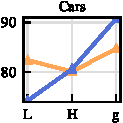
\includegraphics{stamp_Cars.pdf}
  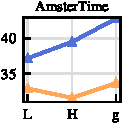
\includegraphics{stamp_AmsterTime.pdf}
  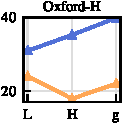
\includegraphics{stamp_Oxford-H.pdf} 
  \caption{
    \textbf{Model scale versus data scale.}
    Evolution of performance as a function of model size for two different pretraining datasets: ImageNet-22k (14M images) and \LaViDa{} (142M images).
    The ViT-g trained on \LaViDa{} surpasses the ViT-g trained on ImageNet-22k on most benchmarks.
  }
\label{fig:scaleperf}
\end{figure*}


\subsection{Loss Components}
We validated the proposed technical improvements in Sec.~\ref{sec:ablation-ibot} by adding them incrementally.
This section analyzes the performance hit observed if we ablate specific loss terms, starting from our best-performing model.
We ablate the importance of the KoLeo loss and the impact of the masked image modeling term.
For both, we report performance on ImageNet-1k using a linear classifier, ADE-20k segmentation using a linear classifier, and nearest-neighbor image retrieval on Oxford-M.
Table~\ref{tab:koleo} shows the impact of using the KoLeo loss.
We see that the instance retrieval performance improves by more than $8\%$, confirming that this term helps spread features in the output space.
At the same time, the other metrics do not suffer from this regularization.
In Table~\ref{tab:ibot}, we show the impact of using the masked image modeling term from iBOT.
This term is critical for dense prediction tasks, leading to almost $3\%$ performance improvement.

\begin{table}[t]
  \begin{subtable}[h]{0.5\linewidth}
    \centering
    \resizebox{0.98\textwidth}{!}{%
    \begin{tabular}{@{}l c cccc@{}}
      \toprule
      KoLeo && INet-1k & Im-A & ADE-20k & Oxford-M \\
      \midrule
      \ding{53}   && 85.3 & 70.6 & 47.2 & 55.6 \\ 
      \checkmark  && 85.8 & 72.8 & 47.1 & 63.9 \\
      \bottomrule
    \end{tabular}
    }
    \caption{Koleo loss}
    \label{tab:koleo}
  \end{subtable}
  \begin{subtable}[h]{0.5\linewidth}
    \centering
    \resizebox{0.98\textwidth}{!}{%
    \begin{tabular}{@{}l c cccc@{}}
      \toprule
      MIM && INet-1k & Im-A & ADE-20k & Oxford-M \\
      \midrule
      \ding{53}   && 85.3 & 72.0 & 44.2 & 64.3 \\ 
      \checkmark  && 85.8 & 72.8 & 47.1 & 63.9 \\
      \bottomrule
    \end{tabular}
    }
    \caption{MIM objective in iBOT}
    \label{tab:ibot}
  \end{subtable}
  \caption{
    \textbf{(a)} Effect of the KoLeo loss term. 
    \textbf{(b)} Effect of the iBOT Masked Image Modeling (MIM) loss term. 
Evaluation performed on ImageNet-\{1k,A\} (classification with linear probe, accuracy \%), ADE-20k (segmentation with linear layer, mIoU) and Oxford-M (image retrieval, mAP). 
Each model is trained on the same number of iterations, that is smaller than our final run.
The KoLeo loss term improves nearest-neighbor search tasks (e.g. retrieval), and the MIM loss improves patch-level tasks (e.g. segmentation). 
  }
  \label{tab:all_ablations}
\end{table}


\subsection{Impact of Knowledge Distillation}
For small architectures, we distill larger models instead of training them from scratch.
We use the distillation procedure described in Sec.~\ref{sec:distill}. 
We evaluate the effectiveness of this approach by comparing a ViT-L/14 trained from scratch with one distilled from a ViT-g/14 over 12 benchmarks in Fig.~\ref{fig:distillation}.
We also report the performance of the ViT-g/14 used for distillation as a topline.
The distilled model outperforms the one trained from scratch on \rtwo{all 12} benchmarks, validating our pretraining approach for small models.

\begin{figure}[t]
  \begin{subfigure}[b]{0.43\linewidth}
    \centering
    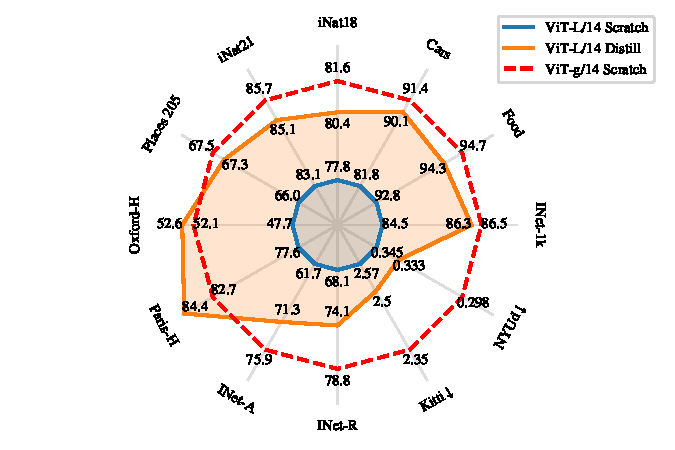
\includegraphics[width=0.98\textwidth,trim=2cm 0 0 0,clip]{ablation_distil_spider.pdf}
    \caption{Comparison on individual metrics}
  \end{subfigure}
  \hfill
  \begin{subfigure}[b]{0.54\linewidth}
    \centering
    \resizebox{0.98\textwidth}{!}{%
    \begin{tabular}{@{}ll c cccc@{}}
      \toprule
      Arch & Method && INet-1k & Segm. & Depth$\downarrow$ & Classif. \\
      \midrule
       \textcolor{gray}{ViT-g/14} & \textcolor{gray}{Scratch} && \textcolor{gray}{86.5} & \textcolor{gray}{73.4} & \textcolor{gray}{1.00} & \textcolor{gray}{92.1} \\
       ViT-L/14 & Scratch && 84.5 & 72.2 & 1.10 & 90.2 \\ 
       ViT-L/14 & Distill && \bf 86.3 & \bf 73.3 & \bf 1.08 & \bf 91.2 \\ 
       \bottomrule
       \\
       \toprule
       Arch & Method && Finegr. & Retriev. & ARSketch & Video \\
       \midrule
       \textcolor{gray}{ViT-g/14} & \textcolor{gray}{Scratch} && \textcolor{gray}{78.3} & \textcolor{gray}{75.2} & \textcolor{gray}{77.0} & \textcolor{gray}{69.3} \\
       ViT-L/14 & Scratch && 75.8 & 71.3 & 69.5 & 67.3 \\ 
       ViT-L/14 & Distill && \bf 77.6 & \bf 76.3 & \bf 74.5 & \bf 67.5 \\ 
      \bottomrule
    \end{tabular}
    }
    \vspace{2em}
  \caption{Averaged metrics on 8 vision tasks}
  \end{subfigure}
  \caption{
    \textbf{Effectiveness of knowledge distillation.}
    Comparison between a ViT-L trained from scratch or distilled from \OURS{} using ViT-g/14.
    For reference, we also report the performance of the ViT-g/14 teacher. We show that a ViT-L model distilled from a frozen ViT-g outperforms a the same model trained from scratch on all benchmarks, sometimes even outperforming the distillation target.
}
  \label{fig:distillation}
\end{figure}


\subsection{Impact of Resolution}
We measure the impact of changing the resolution during the pretraining on the performance of image and patch-level features.
We consider models trained from scratch using a fixed resolution of either $224\times 224$ or $416\times 416$, and a model trained from scratch at $224\times 224$, then resumed for 10k more iterations at $416\times 416$. 
High-resolution training is compute-intensive, so we conduct this ablation on a small setup: a ViT-L/16 trained on ImageNet1k.
In Fig.~\ref{fig:res}, we report the performance of a linear probe on ImageNet-1k and ADE-20k, evaluated at various resolutions.
The model trained on high-resolution images performs best across resolutions, but this comes at a high cost: training at $416$ is \rthree{approximately} $3\times{}$ more compute-intensive than training at $224$. 
On the other hand, training at high resolution for only 10k iterations at the end of the training is almost as good and only requiring a fraction of the compute. 
As a consequence, we include this step at the end of the training rather than training at a high resolution from scratch.

\begin{figure}[t]
  \centering
  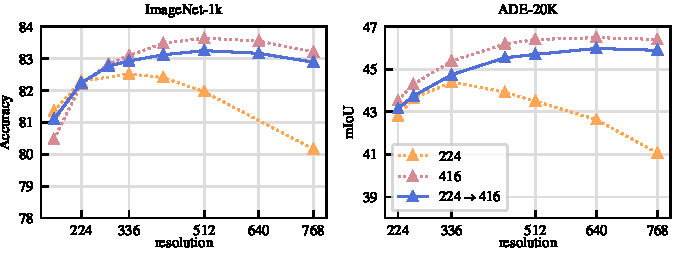
\includegraphics{figure_res.pdf} 
  \caption{
    \textbf{Role of resolution.}
    Performance of ViT-L/16 trained on ImageNet-1k at fixed resolution (``224'' and ``416'') or trained at 224 then 416 for a short duration (``224$\rightarrow$416''). 
    We train linear classifiers on top of frozen features at different resolutions and report Top-1 accuracy on ImageNet and mIoU on ADE-20k. We observe that performing SSL training at high resolution for a short duration achieve behavior and results close to training at the same high resolution for the full training, at a fraction of the cost.
  }
  \label{fig:res}
\end{figure}

